\documentclass[border=8pt]{standalone}
\usepackage[T1]{fontenc}
\usepackage{tikz}
\usetikzlibrary{positioning, arrows.meta, fit, backgrounds}

% ── Colour palette (print-friendly, distinguishable in greyscale) ──
\definecolor{stgI}{HTML}{C6DBEF}
\definecolor{stgII}{HTML}{9ECAE1}
\definecolor{stgIII}{HTML}{6BAED6}
\definecolor{cdraw}{HTML}{2171B5}
\definecolor{afill}{HTML}{FDD0A2}
\definecolor{adraw}{HTML}{E6550D}
\definecolor{ffill}{HTML}{C7E9C0}
\definecolor{fdraw}{HTML}{31A354}
\definecolor{hfill}{HTML}{D9D9D9}
\definecolor{hdraw}{HTML}{636363}
\definecolor{note}{HTML}{525252}

\begin{document}
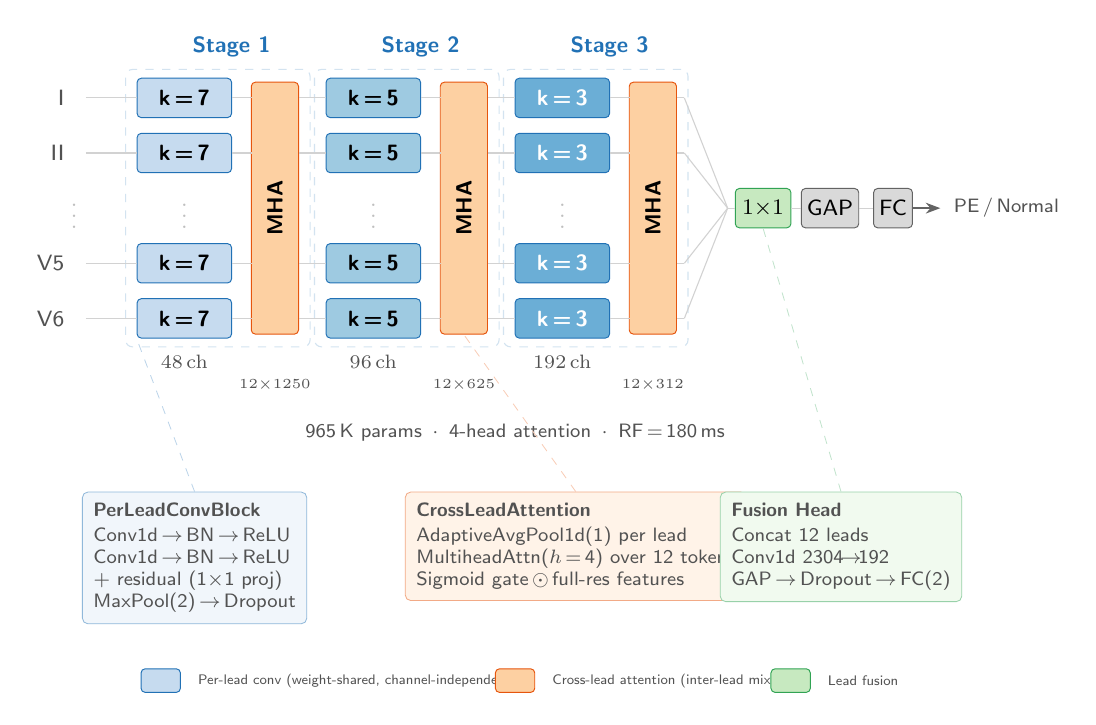
\begin{tikzpicture}[
  x=1cm, y=1cm,
  >=Stealth,
  % ── node styles ──
  cI/.style  ={rectangle, rounded corners=1.5pt,
               minimum width=12mm, minimum height=5mm,
               fill=stgI, draw=cdraw, line width=0.35pt,
               font=\footnotesize\sffamily\bfseries, inner sep=1.5pt},
  cII/.style ={cI, fill=stgII},
  cIII/.style={cI, fill=stgIII, text=white},
  att/.style ={rectangle, rounded corners=1.5pt, minimum width=6mm,
               fill=afill, draw=adraw, line width=0.35pt,
               font=\footnotesize\sffamily\bfseries, inner sep=1.5pt},
  fus/.style ={rectangle, rounded corners=1.5pt, minimum height=5mm,
               fill=ffill, draw=fdraw, line width=0.35pt,
               font=\footnotesize\sffamily, inner sep=2.5pt},
  hd/.style  ={rectangle, rounded corners=1.5pt, minimum height=5mm,
               fill=hfill, draw=hdraw, line width=0.35pt,
               font=\footnotesize\sffamily, inner sep=2pt},
  w/.style   ={draw=gray!35, line width=0.4pt},
  nt/.style  ={font=\scriptsize, text=note},
  sl/.style  ={font=\footnotesize\sffamily\bfseries, text=cdraw},
  dm/.style  ={font=\tiny, text=note},
  % ── detail-box styles ──
  detbox/.style={rectangle, rounded corners=2pt,
                 draw=cdraw!50, fill=stgI!25, line width=0.3pt,
                 inner sep=4pt, font=\scriptsize\sffamily,
                 text=note, align=left},
  detatt/.style={detbox, draw=adraw!50, fill=afill!25},
]

% ════════════════════════════════════════════════════════════════════
%  LEAD LABELS
% ════════════════════════════════════════════════════════════════════
\foreach \lid/\y/\nm in {a/1.4/I, b/0.7/II, c/-0.7/V5, d/-1.4/V6}{
  \node[font=\footnotesize\sffamily, text=note, anchor=east]
    at (-0.1, \y) {\nm};
  \draw[w] (0.05, \y) -- (0.5, \y);
}
\node[font=\footnotesize, text=gray!50] at (-0.1, 0) {$\vdots$};

% ════════════════════════════════════════════════════════════════════
%  STAGE 1 — Per-lead Conv k=7, 48 ch → Cross-lead MHA
% ════════════════════════════════════════════════════════════════════
\foreach \lid/\y in {a/1.4, b/0.7, c/-0.7, d/-1.4}{
  \node[cI] (s1\lid) at (1.3, \y) {k\,=\,7};
  \draw[w] (0.5, \y) -- (s1\lid.west);
  \draw[w] (s1\lid.east) -- (2.15, \y);
}
\node[font=\footnotesize, text=gray!50] at (1.3, 0) {$\vdots$};

\node[att, minimum height=32mm] (m1) at (2.45, 0)
  {\rotatebox{90}{MHA}};
\foreach \y in {1.4, 0.7, -0.7, -1.4}{
  \draw[w] (2.15, \y) -- (m1.west |- 0,\y);
  \draw[w] (m1.east |- 0,\y) -- (2.85, \y);
}

% ════════════════════════════════════════════════════════════════════
%  STAGE 2 — Per-lead Conv k=5, 96 ch → Cross-lead MHA
% ════════════════════════════════════════════════════════════════════
\foreach \lid/\y in {a/1.4, b/0.7, c/-0.7, d/-1.4}{
  \node[cII] (s2\lid) at (3.7, \y) {k\,=\,5};
  \draw[w] (2.85, \y) -- (s2\lid.west);
  \draw[w] (s2\lid.east) -- (4.55, \y);
}
\node[font=\footnotesize, text=gray!50] at (3.7, 0) {$\vdots$};

\node[att, minimum height=32mm] (m2) at (4.85, 0)
  {\rotatebox{90}{MHA}};
\foreach \y in {1.4, 0.7, -0.7, -1.4}{
  \draw[w] (4.55, \y) -- (m2.west |- 0,\y);
  \draw[w] (m2.east |- 0,\y) -- (5.25, \y);
}

% ════════════════════════════════════════════════════════════════════
%  STAGE 3 — Per-lead Conv k=3, 192 ch → Cross-lead MHA
% ════════════════════════════════════════════════════════════════════
\foreach \lid/\y in {a/1.4, b/0.7, c/-0.7, d/-1.4}{
  \node[cIII] (s3\lid) at (6.1, \y) {k\,=\,3};
  \draw[w] (5.25, \y) -- (s3\lid.west);
  \draw[w] (s3\lid.east) -- (6.95, \y);
}
\node[font=\footnotesize, text=gray!50] at (6.1, 0) {$\vdots$};

\node[att, minimum height=32mm] (m3) at (7.25, 0)
  {\rotatebox{90}{MHA}};
\foreach \y in {1.4, 0.7, -0.7, -1.4}{
  \draw[w] (6.95, \y) -- (m3.west |- 0,\y);
  \draw[w] (m3.east |- 0,\y) -- (7.65, \y);
}

% ════════════════════════════════════════════════════════════════════
%  FUSION HEAD — converge 12 leads → 1×1 → GAP → FC → output
% ════════════════════════════════════════════════════════════════════
\foreach \y in {1.4, 0.7, -0.7, -1.4}{
  \draw[w] (7.65, \y) -- (8.2, 0);
}
\node[fus] (f1) at (8.65, 0) {$1{\times}1$};
\draw[w] (8.2, 0) -- (f1.west);

\node[hd] (gap) at (9.5, 0) {GAP};
\draw[w] (f1.east) -- (gap.west);

\node[hd] (fc) at (10.3, 0) {FC};
\draw[w] (gap.east) -- (fc.west);

\draw[->, draw=hdraw, line width=0.5pt] (fc.east) -- (10.9, 0);
\node[nt, anchor=west, font=\scriptsize\sffamily]
  at (10.95, 0) {PE\,/\,Normal};

% ════════════════════════════════════════════════════════════════════
%  ANNOTATIONS — stage labels, channel counts, tensor shapes
% ════════════════════════════════════════════════════════════════════
\node[sl] at (1.9,  2.05) {Stage 1};
\node[sl] at (4.3,  2.05) {Stage 2};
\node[sl] at (6.7,  2.05) {Stage 3};

\node[nt] at (1.3,  -1.95) {48\,ch};
\node[nt] at (3.7,  -1.95) {96\,ch};
\node[nt] at (6.1,  -1.95) {192\,ch};

\node[dm] at (2.45, -2.25) {$12{\times}1250$};
\node[dm] at (4.85, -2.25) {$12{\times}625$};
\node[dm] at (7.25, -2.25) {$12{\times}312$};

\node[nt, font=\scriptsize\sffamily] at (5.5, -2.85)
  {965\,K params\enspace$\cdot$\enspace 4-head attention%
   \enspace$\cdot$\enspace RF\,=\,180\,ms};

% ════════════════════════════════════════════════════════════════════
%  DETAIL INSETS — PerLeadConvBlock + CrossLeadAttention internals
% ════════════════════════════════════════════════════════════════════
\node[detbox, anchor=north west] (dconv) at (0.0, -3.6) {%
  \textbf{PerLeadConvBlock}\\[1pt]
  Conv1d $\!\to\!$ BN $\!\to\!$ ReLU\\
  Conv1d $\!\to\!$ BN $\!\to\!$ ReLU\\
  $+\;$residual (1$\times$1 proj)\\
  MaxPool(2) $\!\to\!$ Dropout};

\node[detatt, anchor=north west] (datt) at (4.1, -3.6) {%
  \textbf{CrossLeadAttention}\\[1pt]
  AdaptiveAvgPool1d(1) per lead\\
  MultiheadAttn($h$\,=\,4) over 12 tokens\\
  Sigmoid gate $\!\odot\!$ full-res features};

\node[detbox, draw=fdraw!50, fill=ffill!25, anchor=north west] (dfuse) at (8.1, -3.6) {%
  \textbf{Fusion Head}\\[1pt]
  Concat 12 leads\\
  Conv1d 2304$\!\to\!$192\\
  GAP $\!\to\!$ Dropout $\!\to\!$ FC(2)};

% dashed arrows linking insets to main diagram
\draw[dashed, draw=cdraw!30, line width=0.3pt]
  (dconv.north) -- (s1d.south west);
\draw[dashed, draw=adraw!30, line width=0.3pt]
  (datt.north) -- (m2.south);
\draw[dashed, draw=fdraw!30, line width=0.3pt]
  (dfuse.north) -- (f1.south);

% ════════════════════════════════════════════════════════════════════
%  LEGEND (compact, bottom)
% ════════════════════════════════════════════════════════════════════
\node[cI,  minimum width=5mm, minimum height=3mm] at (1.0, -6.0) {};
\node[nt, anchor=west, font=\tiny\sffamily] at (1.35, -6.0)
  {Per-lead conv (weight-shared, channel-independent)};

\node[att, minimum width=5mm, minimum height=3mm] at (5.5, -6.0) {};
\node[nt, anchor=west, font=\tiny\sffamily] at (5.85, -6.0)
  {Cross-lead attention (inter-lead mixing)};

\node[fus, minimum width=5mm, minimum height=3mm] at (9.0, -6.0) {};
\node[nt, anchor=west, font=\tiny\sffamily] at (9.35, -6.0)
  {Lead fusion};

% ════════════════════════════════════════════════════════════════════
%  DASHED STAGE GROUPINGS
% ════════════════════════════════════════════════════════════════════
\begin{scope}[on background layer]
  \node[draw=cdraw!20, dashed, rounded corners=2.5pt,
    inner xsep=4pt, inner ysep=3pt,
    fit=(s1a)(s1d)(m1)] {};
  \node[draw=cdraw!20, dashed, rounded corners=2.5pt,
    inner xsep=4pt, inner ysep=3pt,
    fit=(s2a)(s2d)(m2)] {};
  \node[draw=cdraw!20, dashed, rounded corners=2.5pt,
    inner xsep=4pt, inner ysep=3pt,
    fit=(s3a)(s3d)(m3)] {};
\end{scope}

\end{tikzpicture}
\end{document}
